%%%%%%%%%%%%%%%%%%%%%%%%%%%%%%%%%%%%%%%%%
% MUW Poster
% LaTeX Template
% Version 1.0 (31/08/2016)
% (Based on Version 1.0 (31/08/2015) of the Jacobs Portrait Poster
%
% License:
% CC BY-NC-SA 3.0 (http://creativecommons.org/licenses/by-nc-sa/3.0/)
%
% Created by:
% Nicolas Ballarini, CeMSIIS, Medical University of Vienna
% nicoballarini@gmail.com
% http://statistics.msi.meduniwien.ac.at/
%%%%%%%%%%%%%%%%%%%%%%%%%%%%%%%%%%%%%%%%%


\def\footer#1{\def\insertfooter{#1}}
%--------------------------------------------------------------------------------------
%	PACKAGES AND OTHER DOCUMENT CONFIGURATIONS
%--------------------------------------------------------------------------------------

\documentclass[final]{beamer}
\usepackage[scale=1.150]{beamerposter} % Use the beamerposter package
\usetheme{MUWposter}

% Include a logo of your project if desired
\logo{\pgfputat{\pgfxy(-72,105)}{\pgfbox[center,base]{
\includegraphics[width=25cm]{content/logos/Imvia.png}}}}  

\usepackage{multicol}
\usepackage{array}
%The following two are column definitions for the aknowledgements section
\newcolumntype{L}{>{\arraybackslash}m{22cm}}
\newcolumntype{S}{>{\arraybackslash}m{5cm}}
\usepackage{pgf}  
\usepackage{enumitem}
\usepackage{mathtools}
\usepackage{amsmath, amsthm, amssymb, amsfonts}
\usepackage{exscale}
\usepackage{xcolor}
\usepackage{ushort}
\usepackage{setspace}
\usepackage[square,numbers]{natbib}
\usepackage{url}
\usepackage[single=true, macros=true, xspace=true]{acro}
\bibliographystyle{abbrvnat}
\renewcommand{\vec}[1]{\ushort{#1}}
\renewcommand{\vec}[1]{\mathbf{#1}}
\definecolor{default}{RGB}{95,180,229}

%% Acronym definition example using glossaries package
%% \usepackage{acro} is required
%% 
%% For a powerful usage of the acro package look at http://tex.stackexchange.com/questions/135975/how-to-define-an-acronym-by-using-other-acronym-and-print-the-abbreviations-toge

\DeclareAcronym{cnn}{
  short = CNN,
  long = Convolutional Neural Network
}

\DeclareAcronym{pca}{
  short = PCA,
  long = Principal Component Analysis
}

\DeclareAcronym{rcm}{
  short = RCM,
  long = Reflectance Confocal Microscopy
}

\DeclareAcronym{roc}{
  short = ROC,
  long = Receiver Operating Characteristic
}

 
%-----------------------------------------------
%  START Set the colors
%  Uncomment to apply colors you want to use.
%-----------------------------------------------
\colorlet{themecolor}{default}
\usebackgroundtemplate{
\includegraphics{content/figures/Background.pdf}}

%-----------------------------------------------
%  END Set the colors
%-----------------------------------------------


%-----------------------------------------------
%  START Set the width of the columns
%-----------------------------------------------
\setlength{\paperwidth}{33.1in} % A0 width: 46.8in
\setlength{\paperheight}{46.8in} % A0 height: 33.1in
\newlength{\sepmargin}
\newlength{\sepwid}
\newlength{\onecolwid}
\newlength{\twocolwid}
\newlength{\threecolwid}

% The following measures are used for 2 columns
\setlength{\sepmargin}{0.055\paperwidth} % Separation width (white space) between columns
\setlength{\sepwid}{0.03\paperwidth} % Separation width (white space) between columns
\setlength{\onecolwid}{0.43\paperwidth} % Width of one column
\setlength{\twocolwid}{0.9\paperwidth} % Width of two columns

%-----------------------------------------------
%  END Set the width of the columns
%-----------------------------------------------


%--------------------------------------------------------------------------------------
%	TITLE SECTION 
%--------------------------------------------------------------------------------------
\setbeamertemplate{title}[left]
\setbeamertemplate{frametitle}[default][left]

\title{Reflectance Confocal Microscopy and Lentigo: Evaluation of several feature extractors for automatic detection} % Poster title

\author{Romain Cendre, Alamin Mansouri, Jean-Luc Perrot, Elisa Cinotti, Franck Marzani}

\institute{Laboratoire ImViA, EA 7535, Universite de Bourgogne, Dijon, France} % Institution(s)
%--------------------------------------------------------------------------------------

\begin{document}
    \addtobeamertemplate{block end}{}{\vspace*{1ex}} % White space under blocks
    \addtobeamertemplate{block alerted end}{}{\vspace*{0ex}} % White space under highlighted (alert) blocks
    \setlength{\belowcaptionskip}{2ex} % White space under figures
    \setlength\belowdisplayshortskip{1ex} % White space under equations
  
  
    \begin{frame}[t] % The whole poster is enclosed in one beamer frame
    \begin{columns}[t] % The whole poster consists of two major columns
        \begin{column}{\sepmargin}\end{column} % First separator as margin
        
        \begin{column}{\onecolwid} % The first column
            \begin{block}{Introduction}
                \justifying
                Skin cancer is considered as one of the most important pathology of these days, having a daily impact on affected people and strong economic consequence over the world. An early detection of these can helps to prevent most of the repercussions. Many imaging tools have been designed to prevent pathology's of skin.For that purpose, this work focus on \ac{rcm} images for automated diagnosis of Lentigo, a specific type of skin pathology.
               
        	    \begin{figure}
                    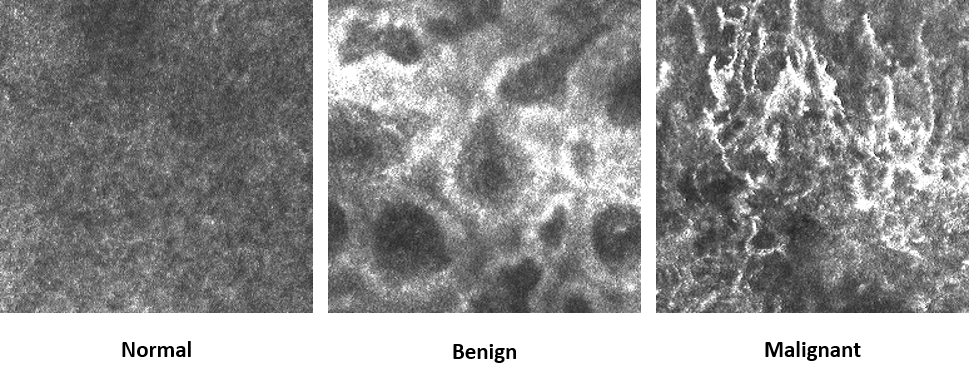
\includegraphics[width=.9\linewidth]{content/figures/Data.png}
				\end{figure}
            \end{block}   
            \begin{block}{Methods}
                \justifying
                This paper evaluate three features extractors : Wavelets \cite{Halimi2017a}, Haralick \cite{Haralick1973}, Deep Features \cite{Litjens2017}.
                \begin{figure}[h]
                    \centering
                    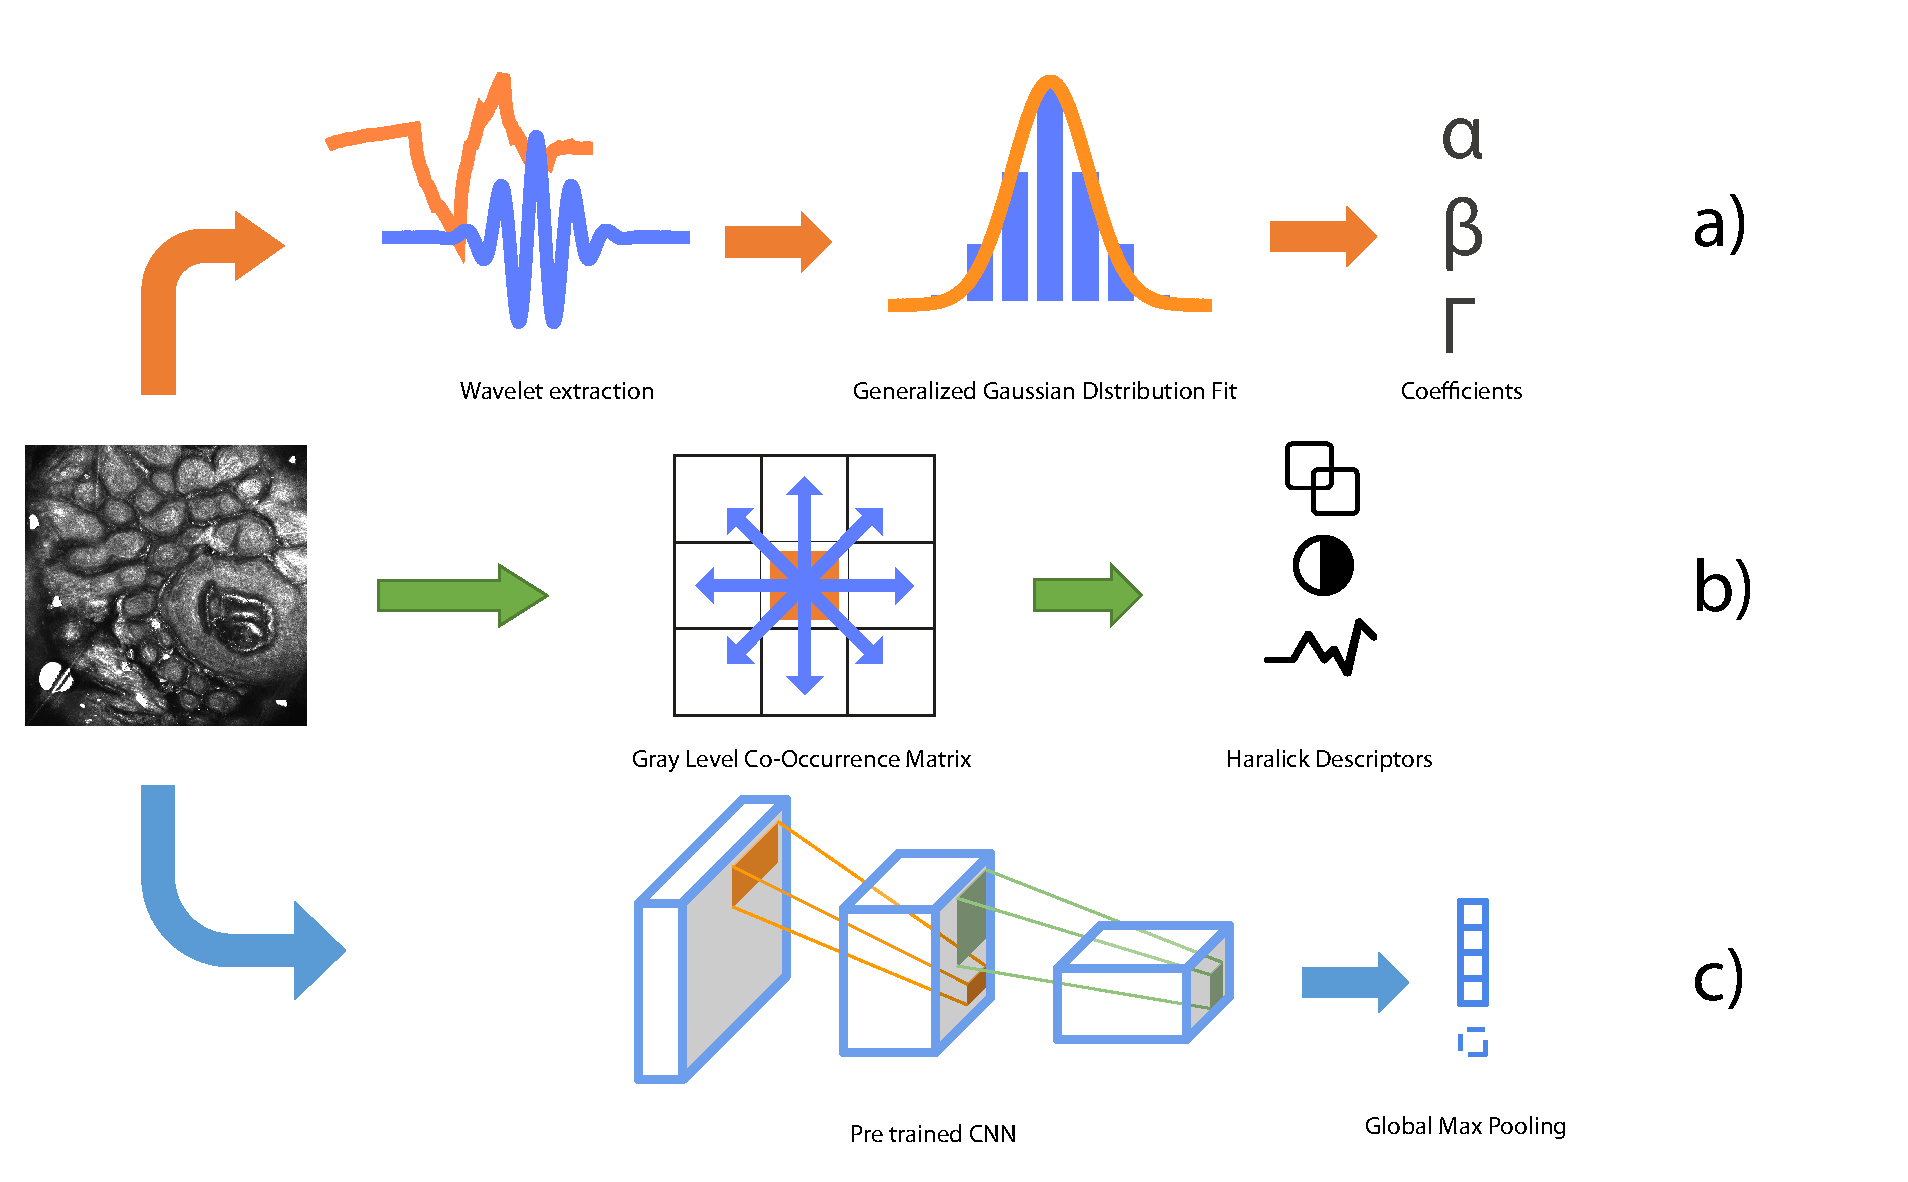
\includegraphics[width=.9\linewidth]{content/figures/Methods.pdf}
                    \label{fig:method_used}
                \end{figure}
                All of these are evaluated using a machine learning pipe. First, features are normalized using a standard score computation. Then, a classification task is performed by a classical SVM using linear kernel.\par
                \begin{figure}[h]
                \centering
                    \includegraphics[width=.9\linewidth]{content/figures/Pipeline.png}
                    \label{fig:pipeline}
                \end{figure}
            \end{block}       
        \end{column}
                      
        \begin{column}{\sepwid}\end{column} % Separate 2 columns
             
        \begin{column}{\onecolwid} %The second column
             
            \begin{block}{Results}
                Uptam, offictibus rem vendipici nonsecest la cullabor moluptas exero quo blam quamentum repudistiam iunda doluptate dolorecta quatem faceaquodit optatum nonse init volori doluptas nam erferch ilique comnihil ma doluptate sanditat ommo temquia nonse sed modicium que vollacillab ius. Uptam, offictibus rem vendipici nonsecest la cullabor moluptas exero quo blam.
                \begin{table}[h]
                    \centering
                    \begin{tabular*}{\textwidth}{l@{\extracolsep{\fill}}lll}
                        \hline
                        Methods & Precision & Recall & F1-Score \\
                        \hline
                        Wavelets & 0.69$\pm$0.04 & 0.69$\pm$0.04 & 0.68$\pm$0.05 \\
                        \hline
                        Haralick & 0.84$\pm$0.02 & 0.83$\pm$0.02 & 0.83$\pm$0.02 \\
                        \hline
                        Deep Learning & 0.89$\pm$0.02 & 0.89$\pm$0.02 & 0.89$\pm$0.02 \\
                        \hline
                    \end{tabular*}
                    \label{table:deep_scores}
                \end{table}
            \end{block}
              
            \begin{block}{ }
    				\begin{figure}
                        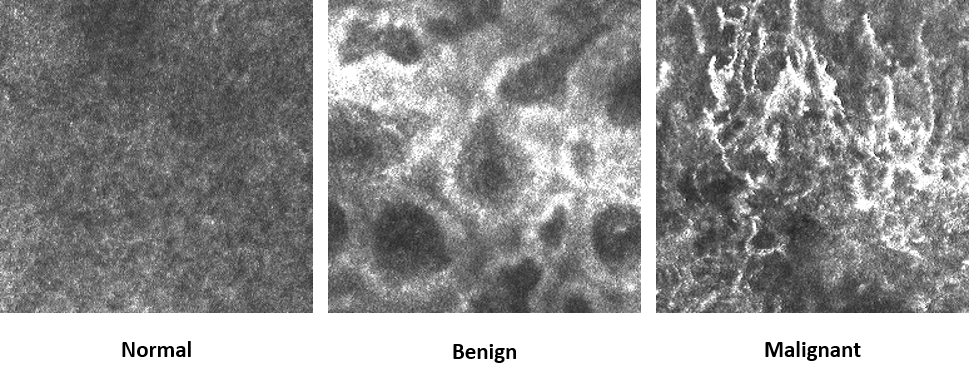
\includegraphics[width=.9\linewidth]{content/figures/Data.png}
    				\end{figure}
                    
                    \begin{multicols}{2}
                    \begin{figure}
                    	\vspace*{-0.95cm}
                        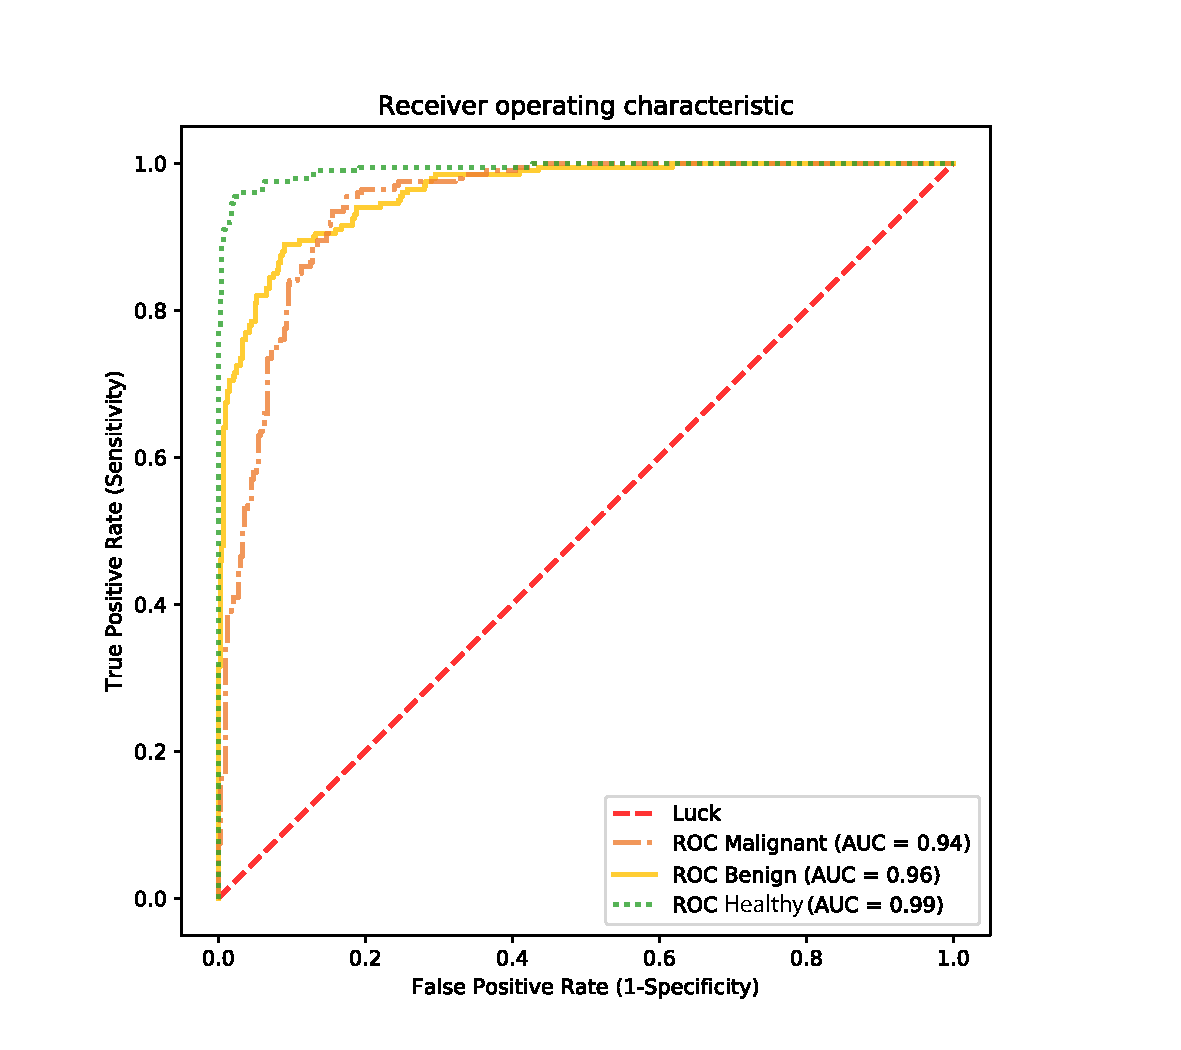
\includegraphics[width=.8\linewidth]{content/figures/ROC.png}
    				\end{figure}
                    \begin{figure}
                    	\vspace*{-0.95cm}
                        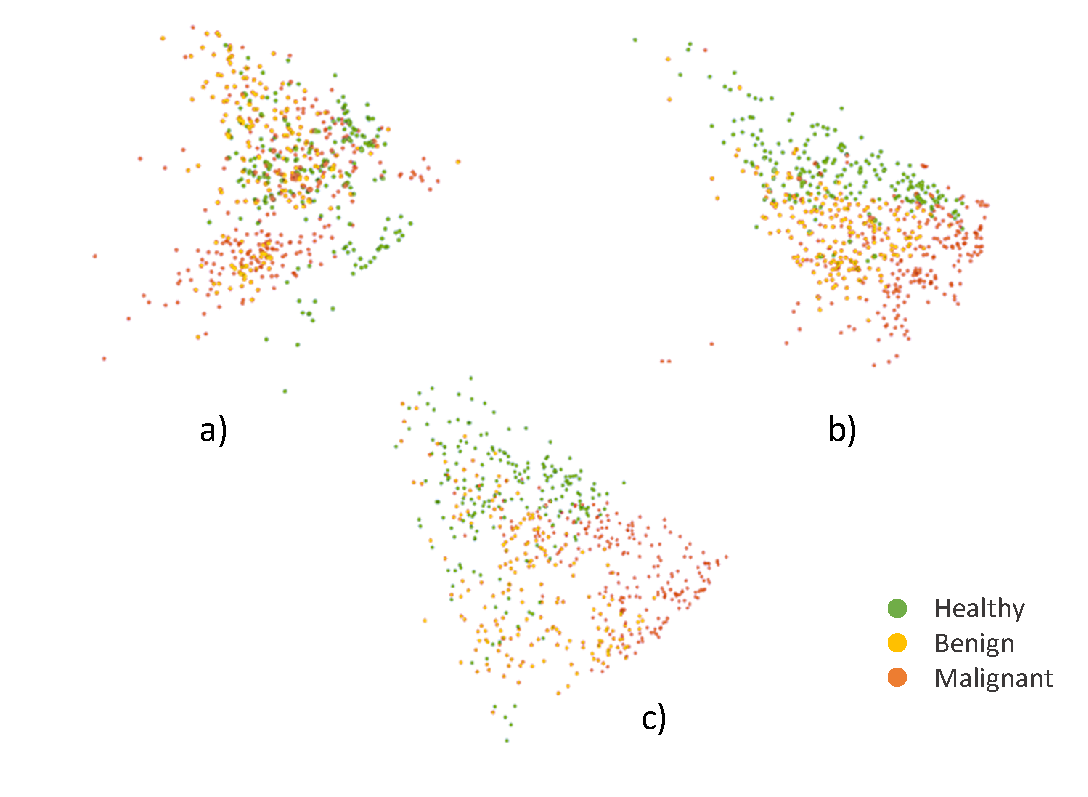
\includegraphics[width=\linewidth]{content/figures/Projection.png}
    				\end{figure}
                    \end{multicols}
            \end{block}
            
    		\begin{block}{Conclusion and Future Work}
            \justifying
              Pertinence of three extraction methods on \ac{rcm} images for diagnosis of Lentigo were evaluated on this study. Haralick and Deep Features approaches shown the most relevant results on classification of patches based on three classes. In further work we should classify whole images using a patch decomposition method or using a Deep Learning end to end solution.
            \end{block}
        \end{column}
          
        \begin{column}{\sepmargin}\end{column} % Separator after second column 
    \end{columns} 
       
    \begin{columns}[t] % Split up the two columns wide column again
      
        \begin{column}{\sepmargin}\end{column} % Separator
        \begin{column}{\onecolwid} % The first column
            \begin{block}{\large Acknowledgements}
                \begin{center}
    				\begin{tabular}{SSL}     				    \includegraphics[width=\linewidth]{content/logos/Bourgogne_small.png}  &		
\includegraphics[width=\linewidth]{content/logos/Europe.png}  &	
    				    \footnotesize This research was supported by the Conseil Regional de Bourgogne Franche-Comte, France and the European Regional Development Fund (ERDF).
    				\end{tabular}
				\end{center}
			\end{block}	
            \vspace*{-0.9cm}
			\begin{alertblock}{\large Contact Information}
                \vspace*{-0.5cm}
				\begin{footnotesize}
					\begin{itemize}
					    \item \textbf{Adress:} ImViA, 9 avenue Alain Savary, 21078 DIJON CEDEX
    					\item \textbf{Phone:} +33612462655
						\item \textbf{Mail:} \href{mailto:romain.cendre@gmail.com}{romain.cendre@gmail.com}
					\end{itemize}
				\end{footnotesize}	
			\end{alertblock}
	    \end{column} % End of the first column
		\begin{column}{\sepwid}\end{column} % Empty spacer column
		\begin{column}{\onecolwid} % Begin a column 
            \begin{block}{\large References}
				\footnotesize 
                \bibliographystyle{unsrt}
                \bibliography{content/bibliography}
            \end{block} 
        \end{column} % End of the second column
            
	    \begin{column}{\sepmargin}\end{column} % Empty spacer column
            
    \end{columns} % End of all the columns in the poster

\end{frame} % End of the enclosing frame
	
\end{document}
